% ============================================================================
% From Agent Loops to Structured Graphs - a reference implementation + study
% Single-column article. Compiles with pdflatex (Overleaf default) or tectonic.
% Figures: upload the five PDF files in ./figures/ with this .tex:
%   fig1_crossover.pdf fig2_parallelism.pdf fig3_cost_vs_correctness.pdf
%   fig4_engine_dag.pdf fig5_scorecard.pdf
% ============================================================================
\documentclass[11pt]{article}

\usepackage[a4paper,margin=1in]{geometry}
\usepackage{graphicx}
\usepackage{booktabs}
\usepackage{amsmath,amssymb}
\usepackage{xcolor}
\usepackage{caption}
\usepackage{enumitem}
\usepackage{microtype}
\usepackage[hidelinks]{hyperref}
\usepackage{titlesec}

\definecolor{ink}{HTML}{1A1D23}
\definecolor{accent}{HTML}{2E86AB}
\hypersetup{colorlinks=true, linkcolor=accent, citecolor=accent, urlcolor=accent}

\graphicspath{{./}{figures/}{../showcase/}}
\captionsetup{font=small,labelfont=bf,labelsep=period}
\titlespacing*{\section}{0pt}{1.4ex plus 1ex minus .2ex}{0.8ex plus .2ex}
\setlist{nosep,leftmargin=1.4em}

\newcommand{\U}{\lvert U\rvert}

\title{\vspace{-2.5em}\textbf{From Agent Loops to Structured Graphs}\\[0.3em]
\large A Reference Implementation and Controlled Study of\\
Graph-Scheduled LLM Agents}

\author{Yash Singh\\
\small IIIT Una\\
\small Code \& data: \url{https://github.com/yashs33244/loops_vs_agents}}

\date{July 2026}

\begin{document}
\maketitle

\begin{abstract}
\noindent
The position paper \emph{From Agent Loops to Structured Graphs}~\cite{sgh2026} argues that
LLM agents should be executed as scheduled directed acyclic graphs (DAGs) rather than as
sequential reason-act loops, but it ships no code and reports no measurements. This work
closes both gaps. First, we build \textbf{SGH}, a from-scratch reference engine in Go
(2{,}655 lines of core code, 2{,}872 lines of tests, standard library only) that realizes the
paper's model: an immutable plan, a ten-state node lifecycle, all-of / any-of join semantics,
a deterministic single-writer scheduler, output-contract validation, a bounded three-level
recovery protocol, and a write-ahead log. Second, we run a controlled loop-versus-graph study
on a real backend codebase with an \emph{objective} pass/fail oracle (a test suite, not an LLM
judge). We observe the crossover the paper predicts: on a small task the graph's fixed
orchestration overhead makes it 50\% slower, but on a larger task the graph finishes
\textbf{23\% faster} in wall-clock by exploiting a measured \textbf{2.1$\times$} parallel
speedup, while always paying a 2--3$\times$ token tax. A companion study on a small model shows
that the obvious way to pay down that tax, trimming context, is \emph{capability-gated}: cutting
tokens by 78\% collapses correctness from 5/5 to 0/5. We argue the practical takeaway is a
dual-path design (loops for trivial work, graphs for parallel-heavy work) with a deterministic
verifier as the one always-safe lever. Every empirical number reported here is traceable to a
released run file; the engine's own statistics come from its source tree and its execution output.
\end{abstract}

\begin{center}
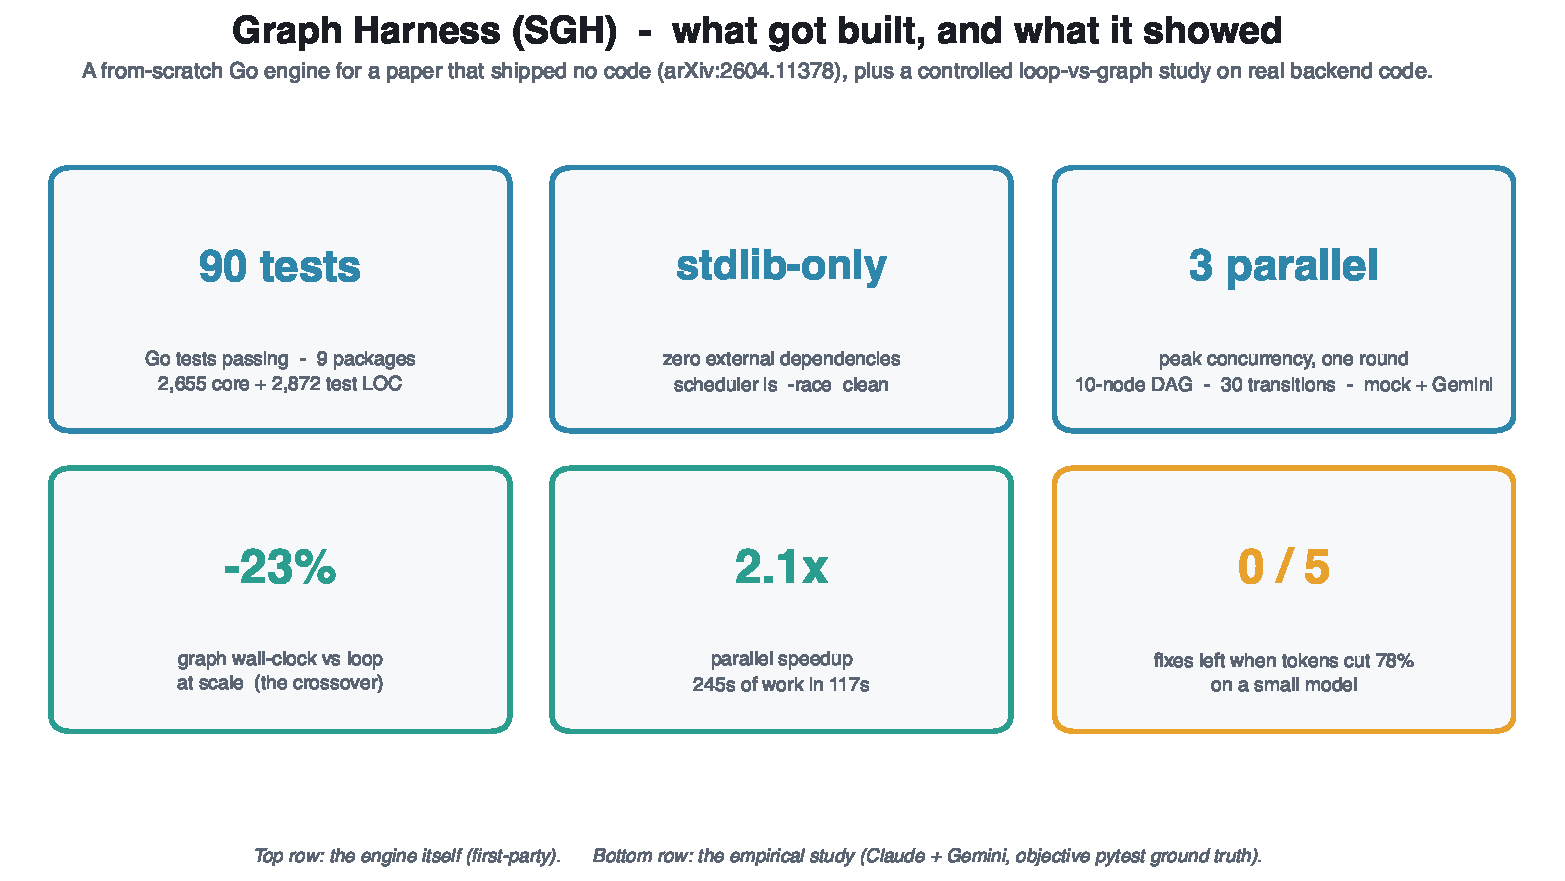
\includegraphics[width=\linewidth]{fig5_scorecard.pdf}
\captionof{figure}{Project at a glance. Top row: the engine itself (first-party).
Bottom row: the empirical study. Every figure in this paper is driven by a released run file.}
\label{fig:scorecard}
\end{center}

\section{Introduction}
The dominant pattern for tool-using LLM agents is the reason-act \emph{loop}: the model emits a
thought, takes one action, observes the result, and repeats~\cite{react}. The loop is simple and
general, but it is also strictly sequential and opaque: every step depends on the last, there is
no place to express that two subtasks are independent, and there is no durable record of why the
agent did what it did. Structured alternatives are not new at the \emph{reasoning} level:
tree-of-thoughts and graph-of-thoughts methods organize a model's intermediate reasoning as a
search tree or DAG~\cite{tot,got}. A recent position paper~\cite{sgh2026} pushes the same
structural idea one level up, to the \emph{orchestration} of tool-using actions: the agent's work
is compiled to a DAG of typed nodes, and a scheduler runs every node whose dependencies are
satisfied. The framing is explicitly scheduler-theoretic, borrowing the vocabulary of
operating-system process scheduling, and it makes concrete predictions about when graphs should
beat loops. It does not, however, provide an implementation or any empirical evidence.

This paper is an experience report that supplies both. Our contributions are:
\begin{itemize}
\item \textbf{A reference engine} (\S\ref{sec:engine}). A small, dependency-free Go implementation
of the paper's execution model, whose scheduler is a single-writer event loop that stays clean
under Go's race detector. It runs the paper's canonical ten-node bug-fix DAG to completion on a
mock backend and on a live LLM provider.
\item \textbf{A controlled study} (\S\ref{sec:method}--\S\ref{sec:results}). A loop-versus-graph
comparison on real backend code at two task scales, plus a cost-lever study on a small model, all
graded by an objective test oracle. We reproduce the predicted crossover and quantify the token
cost of graph execution.
\item \textbf{An honest accounting} (\S\ref{sec:limits}). We are explicit about what the engine
produced versus what the orchestration study produced, and about the narrow scope of the
measurements.
\end{itemize}

\section{Background: scheduling, not looping}
\label{sec:bg}
The central object is a plan $P=(N,E)$, a DAG whose nodes $N$ are typed units of work and whose
edges $E$ are data and ordering dependencies. At any instant the scheduler maintains a
\emph{ready set} $U \subseteq N$: the nodes whose predecessors have all reached a terminal
success state. The loop is the degenerate case $\U = 1$ at all times; a graph scheduler instead
dispatches the entire ready set concurrently, so peak parallelism is $\max_t \U$. Ordering is a
topological sort (Kahn's algorithm~\cite{kahn}); there is no global step counter, only the partial
order the edges impose.

This is deliberately the same abstraction an operating system uses to schedule processes over
cores, and it parallels a third layer: modern models already route each token through only a
sparse subset of their parameters (mixture-of-experts~\cite{moe}), and brain-inspired
sparse-activation architectures push the same ``fire only what matters'' idea
further.\footnote{See the Dragon Hatchling (BDH) line of work on brain-inspired sparse models. We
use it only as conceptual motivation; none of our measurements depend on it.} Three layers, one
idea: do not serialize work that is independent, and do not activate machinery you do not need.
SGH applies that idea at the agent-orchestration layer.

\section{The SGH engine}
\label{sec:engine}
The engine is organized as nine small packages with locked interfaces
(Table~\ref{tab:engine}). The data model (\texttt{plan}) is immutable: a \texttt{Plan} is a
versioned, validated DAG of \texttt{Node}s, each carrying an action reference, a join mode, a
side-effect class, a retry budget, and an output \texttt{Contract}. A node moves through a
ten-state lifecycle: \texttt{pending}, \texttt{ready}, \texttt{running}, \texttt{waiting\_human},
\texttt{blocked}, \texttt{executed}, \texttt{failed\_retryable}, \texttt{failed},
\texttt{cancelled}, \texttt{skipped}. Four of these are terminal (\texttt{executed},
\texttt{failed}, \texttt{cancelled}, \texttt{skipped}); \texttt{failed\_retryable}, by contrast,
re-enters the schedule.

\paragraph{Join semantics.} An \texttt{all\_of} node waits for every predecessor to succeed; an
\texttt{any\_of} node fires as soon as the \emph{first} predecessor succeeds and skips or cancels
its losing siblings. The latter is how the engine expresses ``try fix A or fix B, take whichever
passes the tests first.''

\paragraph{The one invariant.} The scheduler is a \textbf{single-writer event loop}: exactly one
goroutine owns all mutable node state. Worker goroutines only execute a node and post a completion
event back over a channel; the loop applies the event, appends a write-ahead-log entry, recomputes
the ready set, and dispatches the next wave. There are no mutexes on node state and no shared
writes. The scheduler's tests run under Go's race detector and are clean, a concrete and checkable
property rather than a hope.

\paragraph{Validation and recovery.} Before execution, a plan passes five structural checks
(acyclicity, reachability, join arity, side-effect legality, and contract well-formedness). After
each node runs, its output is checked against a lightweight JSON contract (required keys and
types); we deliberately use a deterministic check, not an LLM judge. Failures escalate through a
bounded three-level protocol (\emph{retry} the node, \emph{patch} its inputs, then \emph{replan}
the subgraph), after which the node terminates as \texttt{failed}. The bound guarantees the
protocol always halts. Every state transition is journaled, so a run is fully replayable from its
log.

Figure~\ref{fig:dag} shows the engine's own output on the paper's ten-node bug-fix DAG. The run
produced 30 transition events across 10 scheduler rounds with a peak ready set of $\U=3$; the
grayed \texttt{fix\_B} node is the \texttt{any\_of} loser the scheduler skipped at runtime once
\texttt{fix\_A} passed.

\begin{table}[t]
\centering
\small
\caption{The engine, by package. Standard library only; no external Go modules.}
\label{tab:engine}
\begin{tabular}{@{}ll@{}}
\toprule
\textbf{Package} & \textbf{Responsibility}\\
\midrule
\texttt{plan}      & immutable DAG model: \texttt{Plan}, \texttt{Node}, joins, the 10-state lifecycle\\
\texttt{validate}  & five structural checks + Kahn topological sort\\
\texttt{contract}  & per-node output validation (required keys + types)\\
\texttt{provider}  & LLM backends behind one interface: mock, Claude CLI, Gemini API\\
\texttt{node}      & executor interface: mock, tool, and LLM executors\\
\texttt{wal}       & append-only JSON-lines write-ahead log; replay rebuilds state\\
\texttt{recovery}  & bounded retry, patch, replan escalation\\
\texttt{scheduler} & the single-writer event loop (the heart)\\
\texttt{cmd/sgh}   & the command-line runner\\
\midrule
\multicolumn{2}{@{}l@{}}{\emph{Size:} 2{,}655 core LOC, 2{,}872 test LOC, 90 test functions, scheduler \texttt{-race} clean.}\\
\bottomrule
\end{tabular}
\end{table}

\begin{figure}[t]
\centering
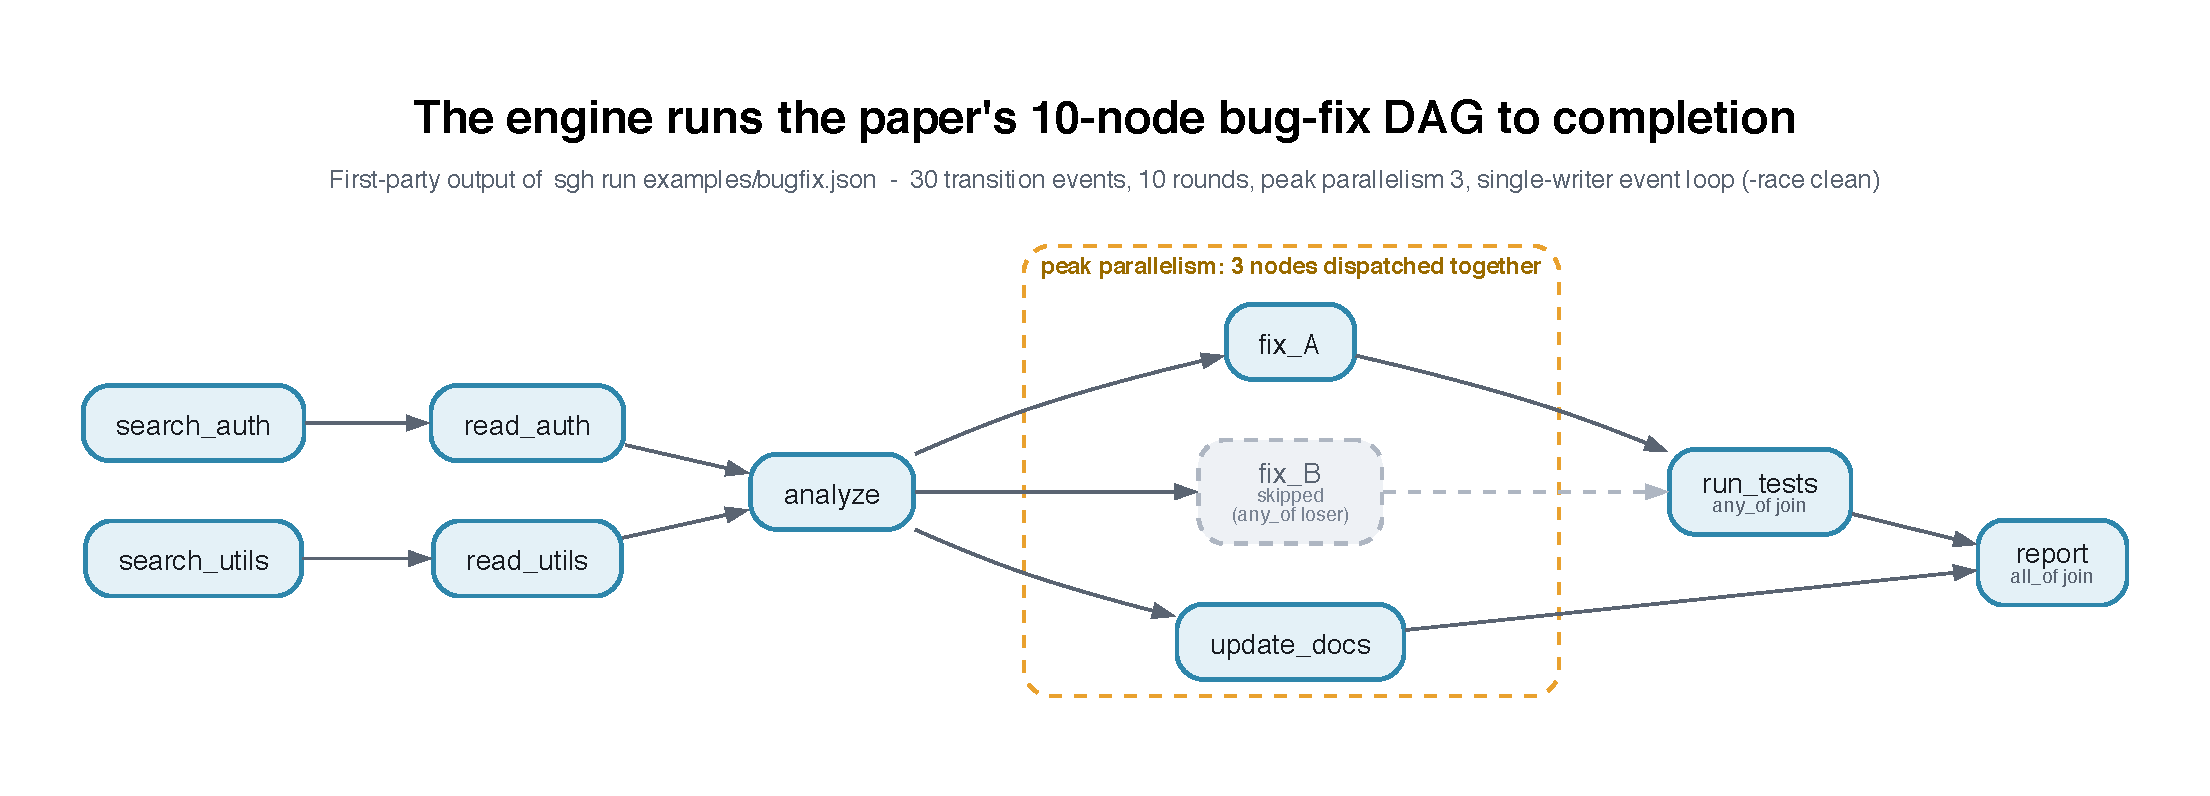
\includegraphics[width=\linewidth]{fig4_engine_dag.pdf}
\caption{First-party output of \texttt{sgh run examples/bugfix.json}: the paper's ten-node
bug-fix DAG executed to a terminal state (rendered by Graphviz from the real dependency
structure). The amber band is the peak-parallelism layer the single-writer loop dispatched in one
round; \texttt{fix\_B} is the \texttt{any\_of} loser, skipped at runtime.}
\label{fig:dag}
\end{figure}

\section{Experimental method}
\label{sec:method}
\paragraph{Codebase and oracle.} All tasks are defined on a real FastAPI backend (an outreach
service with campaigns, chat sessions, repositories, and providers). Correctness is judged by the
project's own \texttt{pytest} suite: an objective, token-free oracle with a fixed baseline
(failing tests) and a fixed target (all passing). No LLM grades another LLM.

\paragraph{Arms.} The \emph{loop} arm is a single ReAct agent that reads, edits, and re-runs tests
until green. The \emph{graph} arm decomposes the task into independent fix-nodes that run in
parallel, followed by a single verify checkpoint (an \texttt{all\_of} or \texttt{any\_of} join).
Both arms use the same model and the same oracle; the only variable is loop versus graph
execution.

\paragraph{Tasks at two scales.} The \emph{small} task is two independent bugs in the chat module
(2 files). The \emph{large} task is a production-hardening pass: seven failing tests spanning
input validation, a broken access-control fix (an insecure direct object reference, IDOR), and
pagination, across five files.

\paragraph{Cost-lever study.} Separately, on the small model \texttt{gemini-3.1-flash-lite}, we
target the five hardening tests from the large task (scored on those five, not the full suite)
under three context regimes: \emph{naive} (full context), \emph{optimized} (scoped context), and
\emph{balanced} (minimal targeted edits). The aim is to measure how context size trades against
tokens and correctness.

\paragraph{What executed what (honesty note).} The loop and graph timing and token figures come
from LLM-agent orchestration: Claude sub-agents for the loop and graph arms, and direct Gemini API
calls structured as nodes for the cost study. The SGH engine of \S\ref{sec:engine} is a separate
reference implementation that executes the same class of DAGs deterministically; we did not yet
route the orchestration study through the engine's scheduler end-to-end. We treat that as future
work (\S\ref{sec:limits}), and we are careful below to attribute each number to its source.

\section{Results}
\label{sec:results}

\subsection{The crossover}
Figure~\ref{fig:crossover} and Table~\ref{tab:cross} give the headline. On the small task the loop
wins: the graph's planning and orchestration overhead is a fixed cost a two-bug task cannot
amortize, so the graph is 50\% slower (112.7\,s vs 75.1\,s) \emph{and} costs 3.0$\times$ the tokens.
On the large task the result flips: the graph finishes \textbf{23\% faster} (116.8\,s vs 152.6\,s)
while costing 2.1$\times$ the tokens. This is the fixed-overhead crossover the paper predicts:
parallelism only pays once there is enough independent work to parallelize. The token tax never
disappears; it is the price of the wall-clock win.

\begin{table}[h]
\centering
\small
\caption{Loop versus graph at two task scales. Both arms reached the same passing state; the only
variable is execution style. Source: \texttt{runs/metrics.json} (small),
\texttt{runs/claude\_arms.json} (large).}
\label{tab:cross}
\begin{tabular}{@{}llrrrr@{}}
\toprule
\textbf{Task} & \textbf{Arm} & \textbf{Wall (s)} & \textbf{Tokens} & \textbf{Token tax} & \textbf{Result}\\
\midrule
Small (2 bugs)  & Loop  & 75.1  & 48{,}287  & 1.0$\times$ & pass\\
Small (2 bugs)  & Graph & 112.7 & 146{,}940 & 3.0$\times$ & pass\\
Large (7 issues)& Loop  & 152.6 & 48{,}364  & 1.0$\times$ & 25/25\\
Large (7 issues)& Graph & \textbf{116.8} & 103{,}453 & 2.1$\times$ & 25/25\\
\bottomrule
\end{tabular}
\end{table}

\begin{figure}[t]
\centering
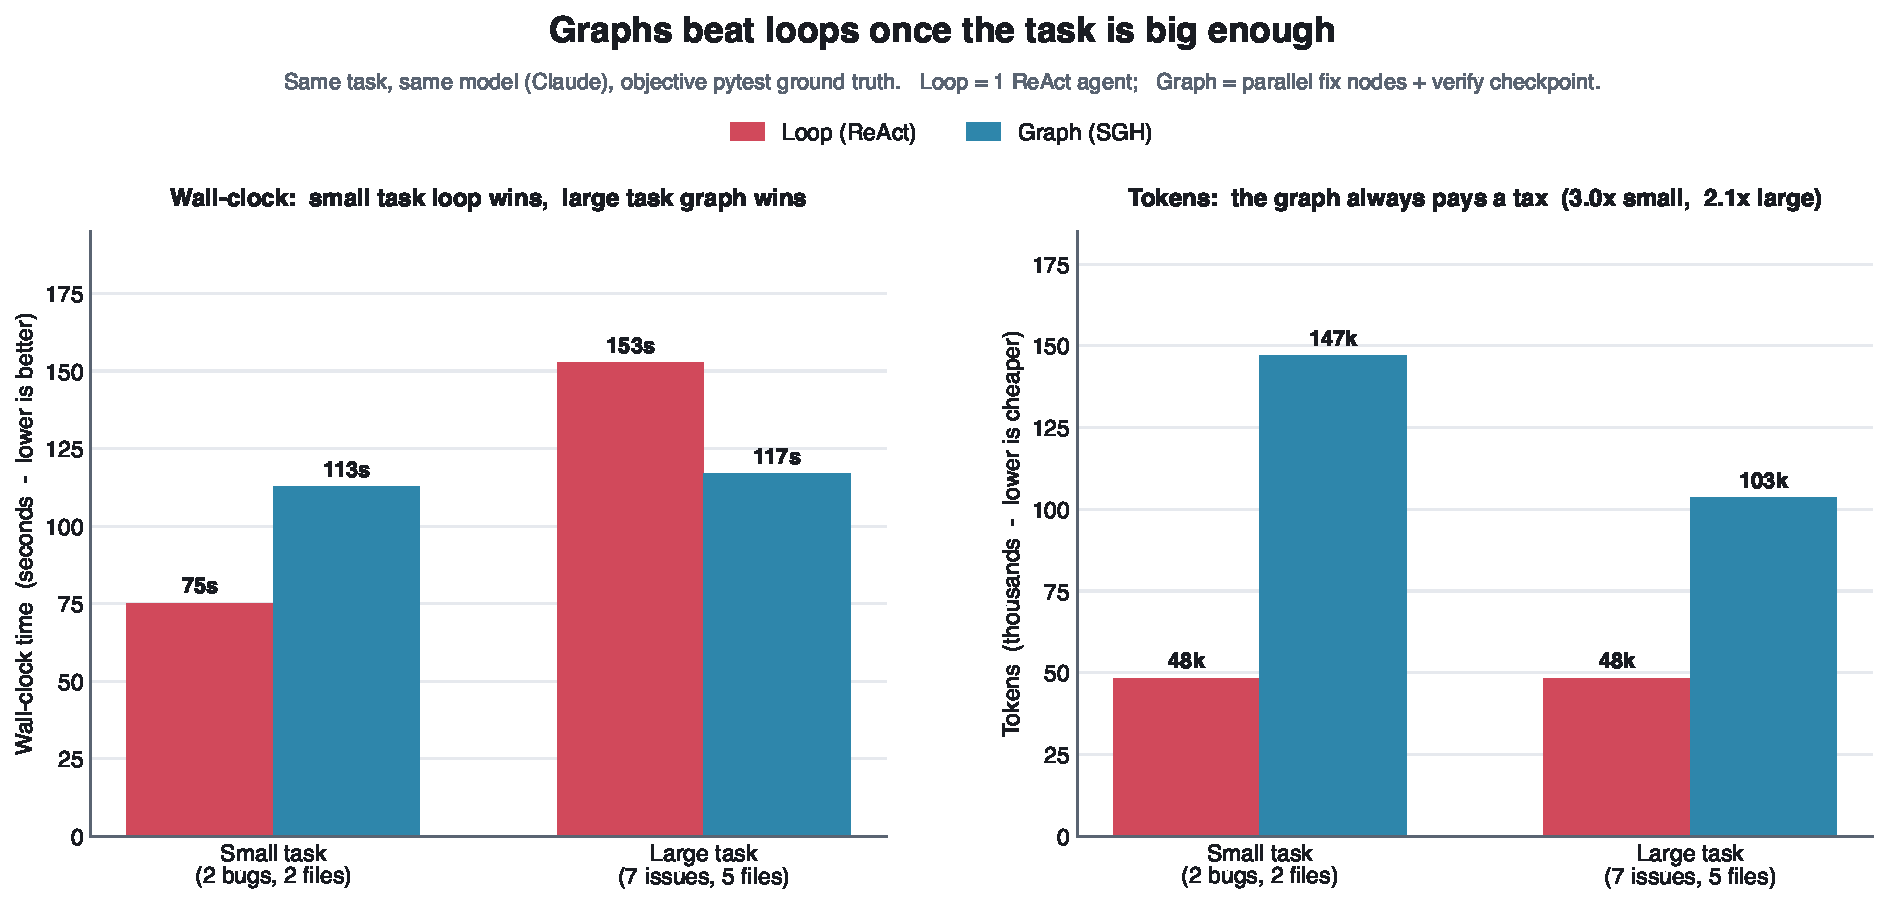
\includegraphics[width=\linewidth]{fig1_crossover.pdf}
\caption{The crossover. Same task, same model (Claude), objective \texttt{pytest} oracle. The graph
loses wall-clock on a tiny task and wins it on a larger one (left), but always pays a token tax
(right).}
\label{fig:crossover}
\end{figure}

\subsection{Where the speedup comes from}
The large-task graph win is not magic; it is parallelism. Figure~\ref{fig:par} is a Gantt chart of
the three fix-nodes the scheduler proved independent and dispatched together. Their measured
durations sum to 245.2\,s of work, but run concurrently they finish in a 116.8\,s makespan, a
\textbf{2.1$\times$} speedup with peak $\U=3$. The ready-set abstraction of \S\ref{sec:bg} is the
mechanism: every node whose dependencies are met runs at once.

\begin{figure}[t]
\centering
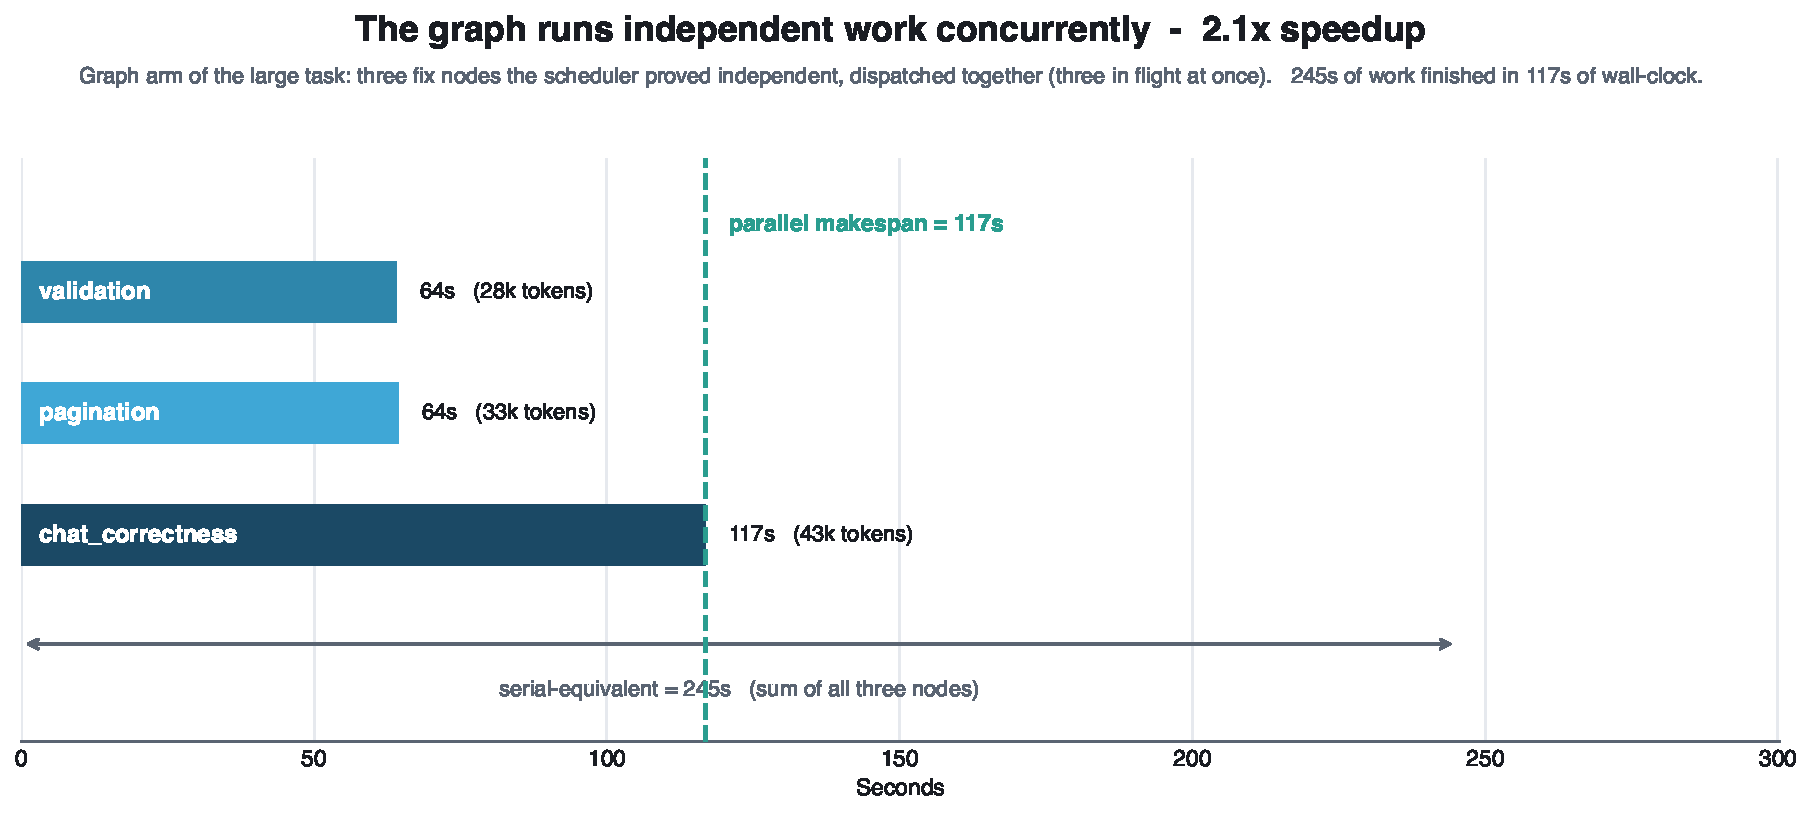
\includegraphics[width=\linewidth]{fig2_parallelism.pdf}
\caption{The graph runs independent work concurrently. Three fix-nodes (real measured durations);
245.2\,s of work completed in a 116.8\,s wall-clock makespan. Source: \texttt{runs/claude\_arms.json}.}
\label{fig:par}
\end{figure}

\subsection{Cheap is not free}
The obvious way to pay down the token tax is to feed each node less context. It works, and it is
dangerous. Figure~\ref{fig:cost} and Table~\ref{tab:gem} show the cost-lever study on a small
model. Trimming context cuts tokens by 66--78\%, but correctness collapses: the \emph{naive}
full-context regime lands all 5 fixes, \emph{optimized} lands 1, and \emph{balanced} lands 0. Part
of the reduction is structural: the \emph{optimized} and \emph{balanced} regimes also drop a
separate LLM verify call and lean on the deterministic oracle instead, so the saving combines
context-scoping with one fewer model call. Either way, on a weak model, context-scoping as a cost
lever is \textbf{capability-gated}: safe on a strong model, ruinous on a small one. The one lever
that is always free is the deterministic verifier; it costs no tokens and never hallucinates a pass.

\begin{table}[h]
\centering
\small
\caption{Cost levers on \texttt{gemini-3.1-flash-lite}. Source: \texttt{runs/gemini\_levers.json}.}
\label{tab:gem}
\begin{tabular}{@{}lrrr@{}}
\toprule
\textbf{Regime} & \textbf{Tokens} & \textbf{Reduction} & \textbf{Fixes landed}\\
\midrule
Naive (full context)      & 22{,}442 & 0\%       & \textbf{5/5}\\
Optimized (scoped)        & 7{,}655  & $-$65.9\% & 1/5\\
Balanced (targeted edits) & 4{,}955  & $-$77.9\% & 0/5\\
\bottomrule
\end{tabular}
\end{table}

\begin{figure}[t]
\centering
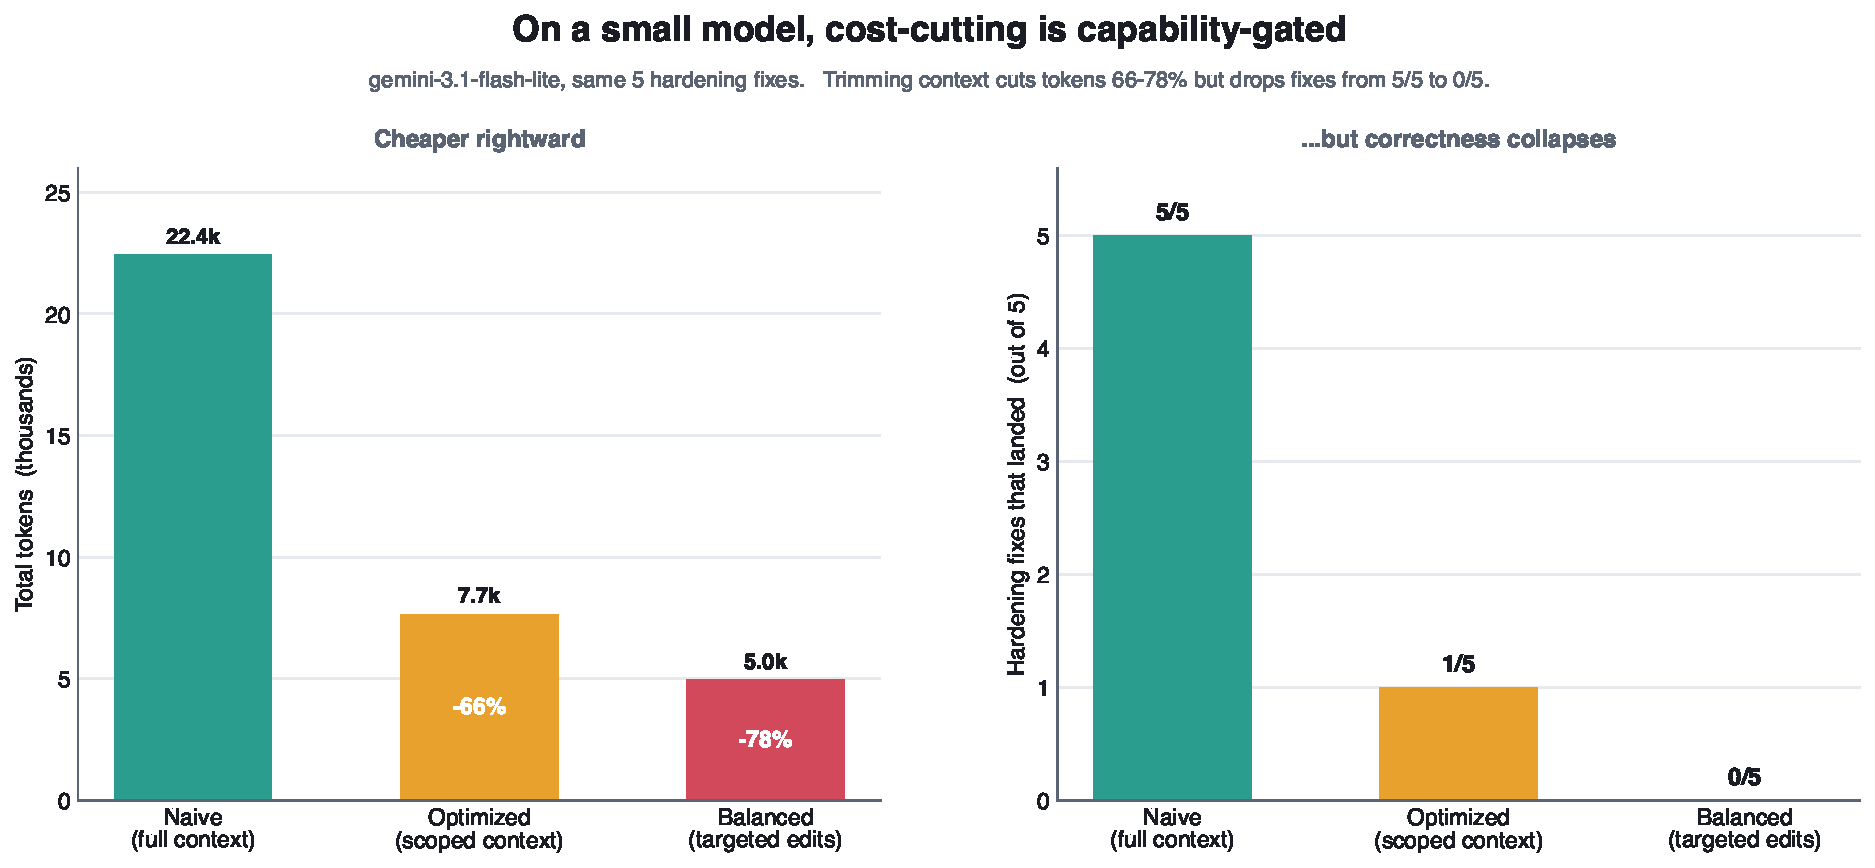
\includegraphics[width=\linewidth]{fig3_cost_vs_correctness.pdf}
\caption{On a small model, cost-cutting is capability-gated. Trimming context (cheaper rightward,
left panel) drops the number of fixes that actually land from 5/5 to 0/5 (right panel).}
\label{fig:cost}
\end{figure}

\section{Discussion}
\label{sec:disc}
Three things follow. \textbf{(1) Graph versus loop is a task-size decision, not a universal win.}
Below the crossover the loop is both faster and cheaper; the right system is dual-path (route
trivial work to a loop and parallel-heavy work to a graph) rather than dogmatically
graph-everything. \textbf{(2) The token tax is structural.} A graph re-establishes context in each
parallel node, so it spends more tokens to buy wall-clock; that trade is only worth it when there
is real parallelism to harvest. \textbf{(3) Determinism is the free lever.} The single safe way to
cut cost without risking correctness is to move judgment out of the model wherever an objective
check exists: here, a test suite as the verify node. This is also why the engine validates
contracts deterministically rather than with an LLM judge. Underneath all three is the scheduling
thesis of \S\ref{sec:bg}: the win comes from not serializing independent work, the same principle
the operating system and sparse models apply one and two layers down.

\section{Limitations and threats to validity}
\label{sec:limits}
We scope the claims narrowly on purpose. The study covers two task scales on a single codebase,
with one run per configuration; it establishes a direction and a crossover, not a precise threshold
or a variance envelope. We report point measurements and do not characterize run-to-run variance,
which for stochastic LLM providers can be substantial. The loop and graph numbers were produced by
LLM-agent orchestration, not by routing the tasks through the SGH scheduler end-to-end, so the
engine and the study validate the same idea from two sides rather than as one closed loop; closing
that loop is the most important next step. The cost-lever result is specific to a small model; on a
strong model we expect context-scoping to be far safer. Finally, token and wall-clock counts are
provider- and load-dependent; we report them as observed, not as guarantees.

\section{Conclusion and future work}
We built the engine that a code-free position paper specified, and we tested its central claim on
real code with an objective oracle. The prediction holds, with a caveat the paper itself names: graphs
beat loops in wall-clock once a task is large enough to amortize their fixed overhead, at a standing
2--3$\times$ token cost. The immediate next steps are to (i) run the loop and graph ablation
\emph{through} the engine's scheduler so the headline numbers are first-party, (ii) add an LLM
planner that compiles an English task into a validated DAG, and (iii) expose the engine as an
HTTP/WebSocket service that streams node transitions live. The code, the run files behind every
figure, and the figure-generation scripts are released at the repository above.

\begin{thebibliography}{9}
\small
\bibitem{sgh2026} \emph{From Agent Loops to Structured Graphs: A Scheduler-Theoretic Framework for
LLM Agent Execution.} arXiv:2604.11378, 2026.
\bibitem{react} S.~Yao, J.~Zhao, D.~Yu, et al. ``ReAct: Synergizing Reasoning and Acting in
Language Models.'' \emph{ICLR}, 2023.
\bibitem{tot} S.~Yao, D.~Yu, J.~Zhao, et al. ``Tree of Thoughts: Deliberate Problem Solving with
Large Language Models.'' \emph{NeurIPS}, 2023.
\bibitem{got} M.~Besta, N.~Blach, A.~Kubicek, et al. ``Graph of Thoughts: Solving Elaborate
Problems with Large Language Models.'' \emph{AAAI}, 2024.
\bibitem{moe} N.~Shazeer, A.~Mirhoseini, K.~Maziarz, et al. ``Outrageously Large Neural Networks:
The Sparsely-Gated Mixture-of-Experts Layer.'' \emph{ICLR}, 2017.
\bibitem{kahn} A.~B. Kahn. ``Topological Sorting of Large Networks.'' \emph{Communications of the
ACM}, 5(11):558--562, 1962.
\end{thebibliography}

\end{document}
